\documentclass{article}
\usepackage{tikz,pgfplots}
\pgfplotsset{compat=1.8}
%\pgfplotsset{colormap={mix}{
%	color(0cm)=(blue);
%	color(1cm)=(green);
%	color(2cm)=(yellow)
%	color(3cm)=(red)}}

\usetikzlibrary{patterns}

\definecolor{diplom1}{rgb}{0.0 0.4 1.0}
\definecolor{diplom2}{rgb}{0.0 0.0 0.6}
\definecolor{diplom3}{RGB}{153,0,0} %unirot
\definecolor{diplom4}{RGB}{232,215,23}
\definecolor{diplom5}{RGB}{51,37,60}

\definecolor{unirot}{RGB}{153,0,0}
\definecolor{unirot_hell}{RGB}{255,228,225}
\definecolor{lightblue}{RGB}{242.2,249.88,255}

\pgfplotsset{colormap={diplom1s}{
       color(0cm)=(white);
       color(1cm)=(diplom1);
       color(10cm)=(diplom1)}}
\pgfplotsset{colormap={diplom2s}{
       color(0cm)=(white);
       color(1cm)=(diplom1);
       color(2cm)=(diplom2)}}



\begin{document}

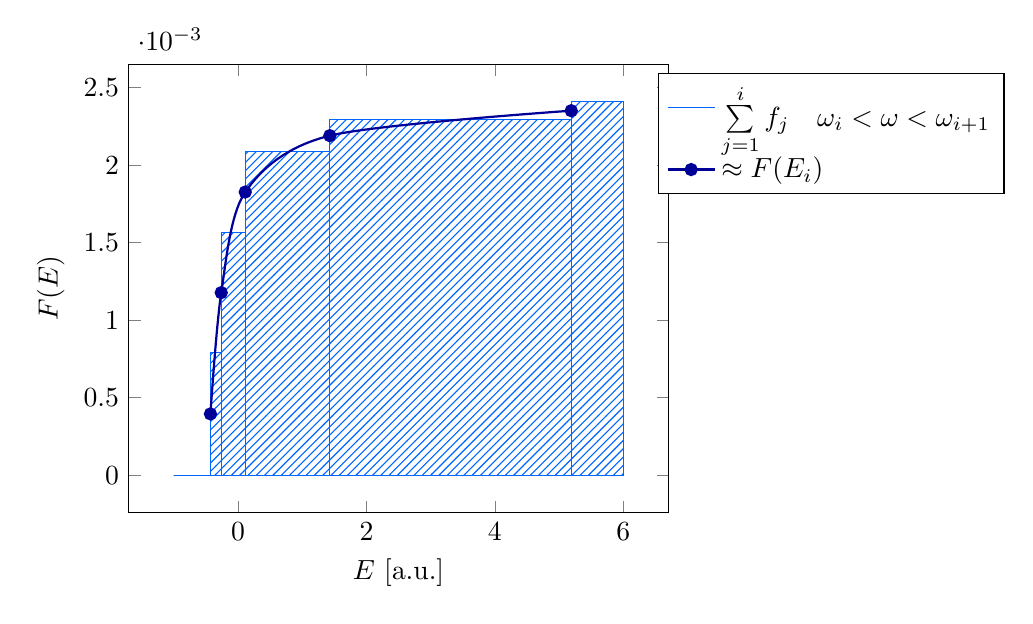
\begin{tikzpicture}
    \begin{axis}[%scale=0.8,
                 domain=-1.0:1.0,
                 samples = 200,
                 %xtick={-3.14159,-1.57089,...,3.14159},
                 %xticklabels={$-\pi$,$-\frac \pi 2$,0,$\frac \pi 2$,$\pi$},
                 cycle list name = exotic,
                 legend style={anchor= north west},
                 legend cell align = left,
                 xlabel= {$E$ [a.u.]},
                 ylabel= {$F(E)$}
                 ]
     \addplot+[domain=-1:-0.42789448546292908,
              diplom1,
              mark = none,
%              forget plot,
              pattern = north east lines,
              pattern color = diplom1
              ]
              {0.0} \closedcycle;
     \addlegendentry{$\sum\limits_{j=1}^{i} f_j \quad \omega_i < \omega < \omega_{i+1}$}
     \addlegendimage{empty legend}
     \addlegendentry{}
     \addplot+[domain=-0.42789448546292908:-0.25969072398345394,
              diplom1,
              mark = none,
              forget plot,
              pattern = north east lines,
              pattern color = diplom1
              ]
              {0.000790314507333} \closedcycle;
     \addplot+[domain=-0.25969072398345394:0.11385089684626037,
              diplom1,
              mark = none,
              forget plot,
              pattern = north east lines,
              pattern color = diplom1
              ]
              {0.00156501308103} \closedcycle;
     \addplot+[domain=0.11385089684626037:1.4305018410002852,
              diplom1,
              mark = none,
              forget plot,
              pattern = north east lines,
              pattern color = diplom1
              ]
              {0.00208878898366} \closedcycle;
     \addplot+[domain=1.4305018410002852:5.1882229137192883,
              diplom1,
              mark = none,
              forget plot,
              pattern = north east lines,
              pattern color = diplom1
              ]
              {0.0022929712885} \closedcycle;
     \addplot+[domain=5.1882229137192883:6,
              diplom1,
              mark = none,
              forget plot,
              pattern = north east lines,
              pattern color = diplom1
              ]
              {0.00241086375443} \closedcycle;
%     \addplot [diplom2, thick,
%               domain=-0.5:6]
%              %{0.001300 * ln(x+2.594992)};
%              {0.001049 * sqrt(x+1.374436)};
%     \addlegendentry{$F(x)= \frac 13 x^3 + x^2 + 2x$}
     %\addplot [diplom3, thick]
     %         {x^4/4 + x};
     \addplot [samples=200,mark=*,thick,smooth,diplom2]
       coordinates {
                   (-0.42789448546292908, 0.0003951572536665)
                   (-0.25969072398345394, 0.0011776637941815)
                   ( 0.11385089684626037, 0.001826901032345)
                   ( 1.4305018410002852, 0.00219088013608)
                   ( 5.1882229137192883, 0.002351917521465)
                   };
     \addlegendentry{$\approx F(E_i)$}
    \end{axis}
\end{tikzpicture}

\end{document}
